\chapter{DISCUSSION \& ANALYSIS}
\section{Introduction}
After clarifying the data collection process and the relevant
procedures adopted for the analysis, this chapter aims to
examine the previously collected data in order to
determine the definitive truth regarding harnessing
AI in higher education. To this end, statistical
tables and graphs will be disclosed. The findings
of this paper are consistent with previous research
results on the practical ways of implementing AI
into humanities, students’ points of view about
their performance while using AI, challenges,
and opportunities. In short, the survey’s results
indicate that students’ academic performance is improved while using AI.
\section{Results}
The data collected from the survey conducted among English university
students revealed compelling insights into the students' perceptions
and experiences with AI-driven tools. The analysis utilized descriptive
statistical techniques to interpret the responses gathered through
the questionnaire. The questionnaire is divided into two main parts:
The first part investigates whether the student's academic performance
has improved or not while using AI-driven methods. The second part is
about the challenges and opportunities faced during using AI for academic studies.
\subsection{The students' academic performance while using AI-driven tools}
% \begin{figure}[h]
% 	\centering
% 	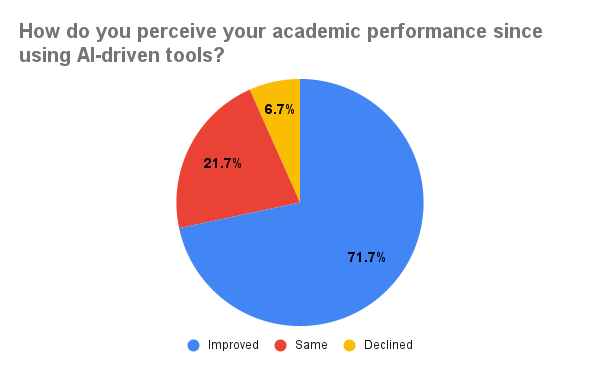
\includegraphics[width=11cm, height=7cm]{./chap4/figures/prf}
% 	\captionof{figure}{perceive academic performance using AI-driven tools}
% \end{figure}

\begin{figure}[h]
	\centering
	\begin{tikzpicture}
		\pie [rotate = 180, explode = 0.1, text=legend, color = {red!40, green!40, blue!30}]
		{71.2/ Improved,
			21.7/ Same,
			6.7/ Declined }
	\end{tikzpicture}
	\captionof{figure}{Perceived academic performance using AI-driven tools}
\end{figure}

After assessing the respondents' opinions on the use of AI-driven tools and students'
academic performance, it is evident that the majority of their academic performance is improved.
The data reported that 71.7\% agreed that AI improves their academic performance.
In addition, 21.7\% of respondents believed that the use of AI did not affect their
academic performance. Whereas 6.7\% showed negative results, believing
that AI affects their academic performance to be declined while using it.
\subsection{The students’ engagement while using AI-driven tools in an academic setting}

% \begin{figure}[H]
% 	\centering
% 	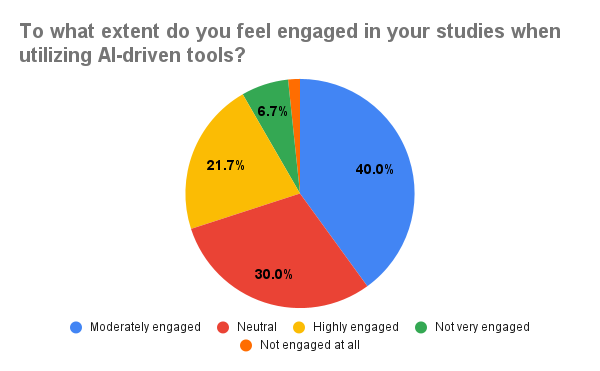
\includegraphics[width=11cm, height=7cm]{./chap4/figures/engagment}
% 	\captionof{figure}{perceive academic engagment using AI-driven tools}
% \end{figure}

\begin{figure}[H]
	\centering
	\begin{tikzpicture}
		\pie [square, text=legend, color = {cyan!40, green!40, yellow!50, red!40, blue!40}]
		{40/ Moderately engaged,
			30/ Neutral,
			21.7/ Highly engaged,
			6.7/ Not very engaged,
			1.7/ Not engaged at all }
	\end{tikzpicture}
	\captionof{figure}{Perceived academic engagement using AI-driven tools}
\end{figure}

The data collected on the extent of student engagement when using AI-driven
tools provides a diverse range of perceptions and experiences.
A significant portion of respondents reported moderately engaged, 40\%,
indicating a level of engagement with these AI-driven tools, with almost equal neutrality,
30\%, suggesting a mixed reception. However, a notable subset of students
reported feeling highly engaged 21.7\%, depicting that these tools can effectively
encourage students to be engaged.
Negatively, the presence of respondents feeling not very engaged 6.7\% and 1.7\% not
engaged at all highlights potential limitations or challenges associated with the
implementation or usage of AI-driven tools.

\subsection{Challenges faced while using AI-driven tools in academic settings}

% \begin{figure}[H]
% 	\centering
% 	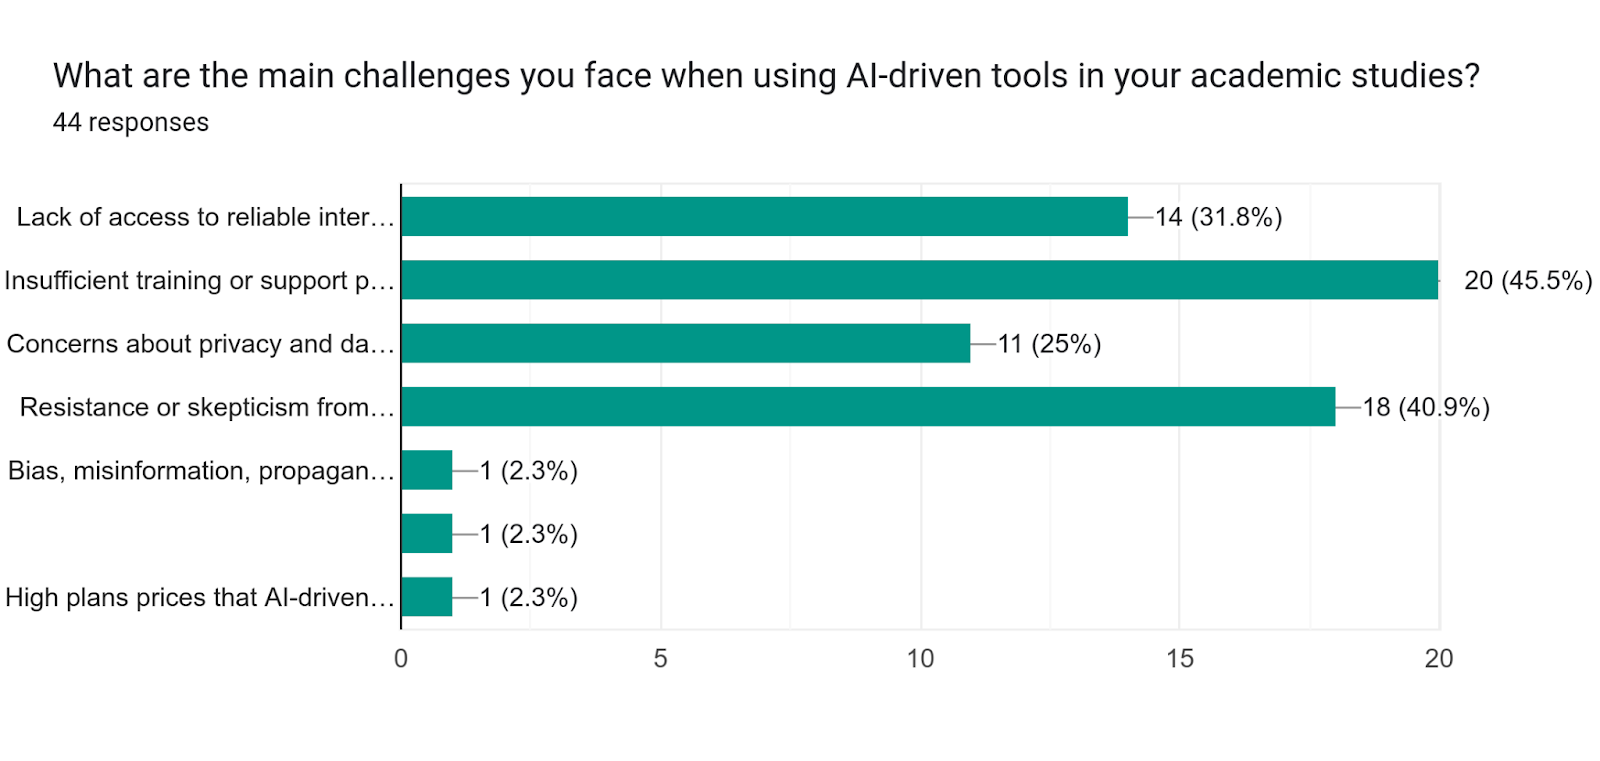
\includegraphics[width=17cm, height=9cm]{./chap4/figures/chall}
% 	\captionof{figure}{challenges faced when using AI-driven tools in academic setting}
% \end{figure}

\begin{figure}[H]
	\centering
	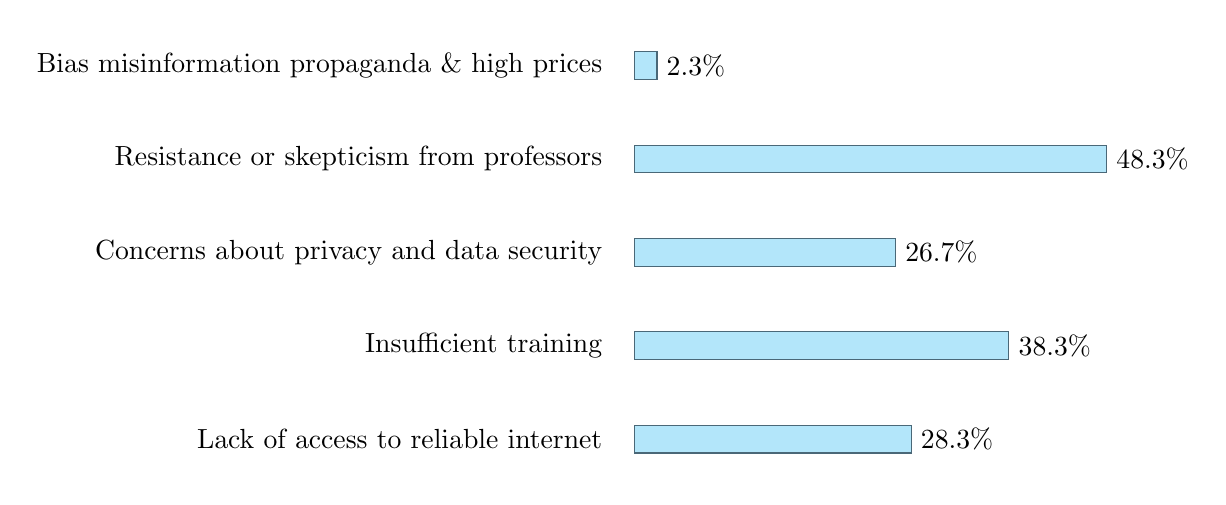
\begin{tikzpicture}
		\begin{axis}[
				xbar,
				y axis line style = { opacity = 0 },
				axis x line       = none,
				tickwidth         = 0pt,
				ytick             = data,
				enlarge y limits  = 0.1,
				symbolic y coords = {Lack of access to reliable internet, Insufficient training, Concerns about privacy and data security, Resistance or skepticism from professors, Bias misinformation propaganda \& high prices},
				nodes near coords={\pgfmathprintnumber{\pgfplotspointmeta}\%},
				nodes near coords align={horizontal},
			]
			\addplot[fill=cyan!30!white, draw=cyan!40!black] coordinates {
					(48.3,Resistance or skepticism from professors)
					(38.3,Insufficient training)
					(28.3,Lack of access to reliable internet)
					(26.7,Concerns about privacy and data security)
					(2.3,Bias misinformation propaganda \& high prices)
				};
		\end{axis}
	\end{tikzpicture}
	\captionof{figure}{challenges faced when using AI-driven tools in academic settings}
\end{figure}
The bar chart shows the results of a survey on the challenges students face when using AI-driven tools in their academic studies.
Out of 60 respondents, the biggest challenge was reported to be the resistance or skepticism from professors toward using AI-driven
tools, with 48.3\% of students selecting that option. Insufficient training is the second challenge faced by 38.8\%.
Following the lack of access to reliable internet, 28.3\% of students reported this as a challenge.
In addition, 26.7\% of students reported concern with their privacy and data security matters. At the same time,
2.3\% was bias, misinformation, propaganda in the AI tools, and high prices of the AI-driven tools.
\subsection{AI-driven tools and opportunities for improving learning experiences in the humanities }
% \begin{figure}[H]
% 	\centering
% 	\captionof{figure}{AI-driven tools and oppu}
% 	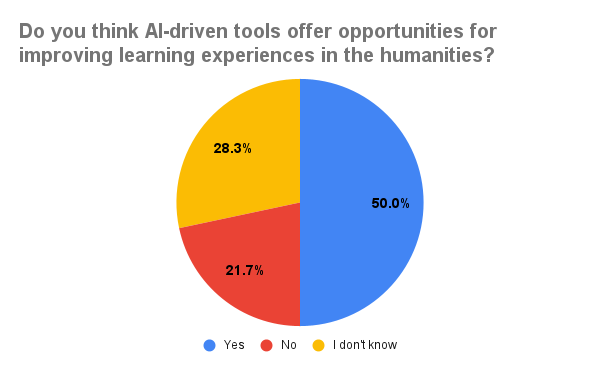
\includegraphics[width=11cm, height=7cm]{./chap4/figures/op.png}
% \end{figure}

\begin{figure}[h]
	\centering
	\begin{tikzpicture}
		\pie [rotate=180, explode=0.1, text=legend, color = {cyan!40, green!40, yellow!50,}]
		{
			50/ Yes,
			21.7/ No,
			28.3/ I don't know
		}
	\end{tikzpicture}
	\captionof{figure}{AI and opportunities}
\end{figure}
The majority of English university students reported that 50\% of AI-driven tools offer opportunities for enhancing learning experiences in the humanities.
In addition, 28.3\% report the ignorance of the opportunities that AI-driven tools offer.
On the other hand, 21.7\% reported that AI-driven tools offer an opportunity to enhance the learning experience within the humanities setting.

Those who answered yes a question were asked to get some examples from students
to understand what kind of opportunities AI-driven tools can offer to enhance the learning experiences,
and the answers were as follows:

% 1st resp
\resp{1}{AI-driven tools in higher education could enhance personalized learning
	through adaptive learning platforms and virtual
	tutoring, and improve research with data analysis tools.}
% 2nd resp
\resp{2}{Research Assistance: AI can assist
	researchers in analyzing vast amounts of
	data, generating hypotheses, and identifying trends,
	accelerating the pace of discovery.}
% 3rd resp
\resp{3}{It can help students be more self-reliant
	and seek knowledge wherever and whenever they want to.}
%4rd resp 
\resp{4}{Making student more used to communicate with chat
	bot ai characters when they can't find native speakers to communicate with.}
%5th resp
\resp{5}{It helps you correct some mistakes and learn from them.
	It elevates your writing and information base and limit their context.}

As it is shown the majority of english students to claim that AI-driven tools can
help students to boost their productivity through analysing the data for researcheres
and provide personalized learning through adaptive learning platforms and virtual tutoring.

\section{Discussion}
It is important to restate the current study's goals and research 
hypothesis before delving into the research findings and discussion.
As mentioned in the introduction, the primary aim of this paper is 
to assess English students' attitudes toward using AI-driven tools
to improve their academic performance and learning experiences. 
Consequently, the recent study has significantly contributed to 
validating or refuting the hypotheses stated in the previous chapter. 
These hypotheses were as follows:
\begin{itemize}
	\item AI-driven tools are singificantly fostering engagment in academic setting.
	\item AI-driven tools are significantly improving academic performance.
	\item There are challenges and opportunities are associated with using AI in higher education
	      in Morocco, specifically in the humanities
\end{itemize}
The current study's findings strongly demonstrate students' positive 
attitudes toward using AI-driven tools as learning aids. 
Precise questions were asked to explore the students' perceptions of the use of AI-driven tools.

Firstly, the findings reveal a significant 40\% 
increase in student engagement when utilizing AI technologies. 
The data collected from English university students strongly 
supports the idea that AI can effectively enhance student engagement, 
fostering a more interactive and dynamic learning environment. 
This aligns with existing literature that emphasizes 
the role of technology in promoting active participation among students.


Secondly, the research results demonstrate a positive correlation 
between using AI-driven tools and students' academic performance. 
As per the data, 71\% of participants believed that AI-driven tools improved their academic performance.
Similarly, a related study by \citep{mohammed_exploring_2023} demonstrated 
that AI-driven tools can effectively enhance academic performance and foster engagement. 
Results showed that most respondents agreed that \say{ChatGPT} motivates and 
engages students by offering access to many resources and improving academic performance.


Furthermore, the research findings shed light on students' challenges 
when utilizing AI-driven tools in educational settings. According to
the participants, these challenges offer valuable insights into the
practical obstacles associated with implementing AI technologies in
learning environments. Issues such as technical difficulties, lack
of training, resistance or skepticism of professors, and concerns
regarding data privacy and security emerge as significant hurdles
that need to be addressed to ensure the effective utilization of AI in education.


Finally, the research results highlight the opportunities presented
by AI-driven tools for transforming learning experiences in the humanities.
By exploring students' perspectives and experiences with AI technologies,
the study uncovers the potential for personalized learning, adaptive tutoring,
and data analysis to help researchers with their vast amount of data.
These opportunities align with the broader literature on the transformative
impact of AI in education, emphasizing technology's role in facilitating
innovative and tailored learning experiences. Leveraging these opportunities
can empower educators to create engaging, effective, and personalized learning
environments that cater to the diverse needs of students in the humanities.
\section{Conclusion}

Throughout this chapter, we have conducted an ongoing study related to
students' attitudes toward the use of AI-driven tools as a learning
tool to enhance learning experiences within academic settings. The
aim was to present and discuss the study's findings in depth.
In addition, this study sought to validate or reject the formulated
hypotheses mentioned in the methodology chapter, correlate the
concluded findings with the paper's literature review and see
how far it converges or diverges from it. The final chapter
will discuss the implications and the limitations of this
study. Finally, it would cover an inclusive summary of the
research paper and serve as a springboard to a more in-depth analysis.

 
